\subsection{Path-space framework}
Given a volume containing quantity $B$ randomly distributed scatterers with configuration $O$, the scattered field of incident light can be written as sums of contributions from all possible paths traveled within the medium. The set of all ordered sequences:
%
\begin{equation} 
    \overset{\rightharpoonup}{\mathbf{x}} = \mathbf{x_0} \rightarrow \mathbf{x_1} \rightarrow ... \rightarrow \mathbf{x_{B+1}}, B \in [0, \infty)
\end{equation}

Let $\mu$ be the change in complex amplitude for a chosen path segment. The speckle mean and covariance calculated for the set of enumerable paths passing through $\mathbf{x_1}...\mathbf{x_B}$ are:
%
\begin{equation}
    m(\overset{\rightharpoonup}{\mathbf{x}}) = \mathbb{E}_O[ u(\overset{\rightharpoonup}{\mathbf{x}}) ] = \mathbb{E}_O \bigg[ \sum \mu(\overset{\rightharpoonup}{\mathbf{x}}) \bigg],
\end{equation}

\begin{equation}
    \mathcal{C}(\overset{\rightharpoonup}{\mathbf{x}}^1,\overset{\rightharpoonup}{\mathbf{x}}^2) = \mathbb{E}_O[ u(\overset{\rightharpoonup}{\mathbf{x}}^1) u(\overset{\rightharpoonup}{\mathbf{x}}^2)^*  - m(\overset{\rightharpoonup}{\mathbf{x}}^1) m(\overset{\rightharpoonup}{\mathbf{x}}^2)^*].
\end{equation}

% Calculating the expected value and covariance is intractable for real materials due to the massive number of particles. A solution is to treat the material as a continuum by considering its density $\zeta(\mathbf{x})$ and its distribution and physical properties of scatterers such as size and refractive properties. These effects are abstracted using three coefficients: the absorption and scattering coefficients ($\sigma_a, \sigma_s$), and their sum, the attenuation coefficient $\sigma$:

% \begin{equation}
%         \sigma_s(\mathbf{x}) = \tilde{N} c_s, \; \sigma_a(\mathbf{x}) = \tilde{N} c_a + \sigma_a^{med}
% \end{equation}


% where $c_a, c_s$ are the scattering and absorption cross-sections denoting the energy scattered or absorbed when light is incident upon a particle, $\tilde{N}$ is the expected number of particles per unit volume, and $\sigma_a^{med}$ is the scattering coefficient of the host medium surrounding each scatterer. 
Given two light sources and two sensors each located at $\mathbf{i_1}, \mathbf{i_2}, \mathbf{v_1}, \mathbf{v_2}$ respectively, the covariance can be written as volume integrals over all possible path pairs by swapping the order of the expectation and sum:
%
\begin{equation}
    \mathcal{C}_{\mathbf{v_1},\mathbf{v_2}}^{\mathbf{i_1},\mathbf{i_2}} = \int \int p(\overset{\rightharpoonup}{\mathbf{x}}^1,\overset{\rightharpoonup}{\mathbf{x}}^2) \mu(\overset{\rightharpoonup}{\mathbf{x}}^1) \mu(\overset{\rightharpoonup}{\mathbf{x}}^2)^* \; d\overset{\rightharpoonup}{\mathbf{x}}^1 d\overset{\rightharpoonup}{\mathbf{x}}^2 - m_{\mathbf{v_1}}^{\mathbf{i_1}} m_{\mathbf{v_2}}^{\mathbf{i_2}*}
    \label{eqn:corr_theoretical}
\end{equation}
%
where $p(\overset{\rightharpoonup}{\mathbf{x}}^1,\overset{\rightharpoonup}{\mathbf{x}}^2)$ is the probability all nodes on both $\overset{\rightharpoonup}{\mathbf{x}}^1$ and $\overset{\rightharpoonup}{\mathbf{x}}^2$ are included in the same particle configuration. Acquiring single-scattering speckle correlations requires choosing the source and sensor pairs locations and evaluating Equation \ref{eqn:corr_theoretical} so measurements are beyond the memory effect range and the multi-scattering path contributions cancel due to random phase. This means $m_{\mathbf{v_1}}^{\mathbf{i_1}} m_{\mathbf{v_2}}^{\mathbf{i_2}*} \approx 0$, and only the integral must be computed.

Returning to the path space framework, given the volume in Figure \ref{fig:2}b, consider a single-scattering path containing only one particle: $\mathbf{i_1} \rightarrow \mathbf{x_b} \rightarrow \mathbf{v_1}$. Ignoring attenuation, the field produced by all scatterers can be expressed
%
\begin{equation}
    u_{\mathbf{i_1}}^{\mathbf{v_1}} \propto \overline{s}_{\mathbf{i_1}}^{\mathbf{v_1}} \sum_{b=1}^B e^{jk(\mathbf{i_1} - \mathbf{v_1}) \cdot \mathbf{x_b}}.
\end{equation}
%
where $\overline{s}_{\mathbf{i_1}}^{\mathbf{v_1}}$ is the square root of the scattering phase function since the phase function is defined for intensity, and amplitude is considered here. Another field $u_{\mathbf{i_1}}^{\mathbf{v_1}}$ will be produced by the other light-sensor pair. The correlation is then the expectation of the product of $u_{\mathbf{i_1}}^{\mathbf{v_1}}$ with $u_{\mathbf{i_2}}^{\mathbf{v_2}*}$ over all possible instantiations. The correlation in terms of a volume integral and the scattering coefficient $\sigma_s$ is
%
\begin{equation}
    \mathcal{C}_{\mathbf{v_1},\mathbf{v_2}}^{\mathbf{i_1},\mathbf{i_2}} \propto \overline{s}_{\mathbf{i_1}}^{\mathbf{v_1}} \overline{s}_{\mathbf{i_2}}^{\mathbf{v_2}} \sigma_s \int_\mathcal{V} e^{jk((\mathbf{i_1} - \mathbf{v_1}) - (\mathbf{i_2} - \mathbf{v_2})) \cdot \mathbf{x}} d \mathbf{x}.
\end{equation}

Single-scattering correlation is maximized when the complex exponential argument is zero. Define $\vec{\omega} = (\mathbf{i_1} - \mathbf{v_1}) - (\mathbf{i_2} - \mathbf{v_2})$. If the sources and sensors are placed symmetrically about the z (depth) axis, only $\omega_z$ is nonzero. $\omega_z$ is minimized by choosing $\mathbf{i_1,i_2,v_1,v_2}$ such that both $\mathbf{i_1} - \mathbf{i_2}$ and $\mathbf{v_2} - \mathbf{v_1}$ are as small as possible. The goal of our research is to find an imaging configuration that satisfies this condition.
%
\begin{figure}
    \centering
    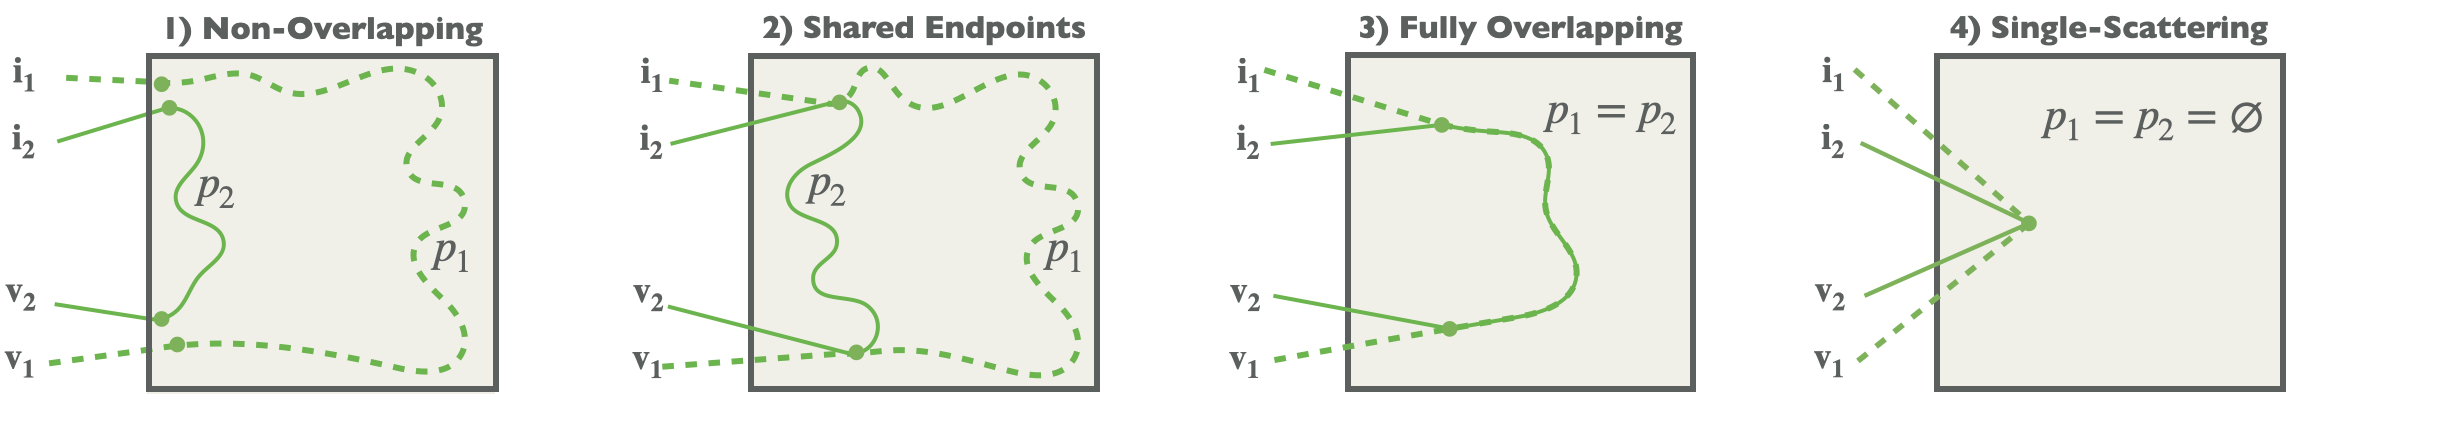
\includegraphics[width=\textwidth]{figures/path_types.png}
    \caption{Scattered light paths can be generally categorized as one of four types, with only type 4 making significant contributions to speckle correlation. Paths types 1 and 2 have no overlap, meaning their phases are random and cancel in expectation. Paths of type 3 generally have non-zero correlation, but their contributions are smaller than those of type 4 (single-scattering paths).}
    \label{fig:path_types}
\end{figure}

\subsection{Single-scattering approximation for speckle correlation}
Consider a volume of scattering particles with configuration $O$. Define $I^{\uvec{i}}(\uvec{v})$ as the intensity scattered in direction $\vec{v}$ by a material illuminated from direction $\vec{i}$. Assuming the material is illuminated from two directions $\uvec{i}^1, \uvec{i}^2$, and light is observed from two directions $\uvec{v}^1, \uvec{v}^2$ the speckle covariance is
%
\begin{equation}
    \mathcal{C}_{\uvec{v}^1,\uvec{v}^2}^{\uvec{i}^1,\uvec{i}^2} \equiv \mathbb{E}_O\Big[I^{\uvec{i}^1}(\uvec{v}^1) \cdot I^{\uvec{i}^2}(\uvec{v}^2)\Big] - \mathbb{E}_O\Big[I^{\uvec{i}^1}(\uvec{v}^1)\Big] \cdot \mathbb{E}_O\Big[I^{\uvec{i}^2}(\uvec{v}^2)\Big]
    \label{eqn:correlation}
\end{equation}
%
where the expected value is evaluated over multiple instantiations of the medium $o \in O$.
The memory effect states that two speckle fields created from similar illumination directions are shifted, correlated versions of each other. Namely, for a small displacement $\Delta = \uvec{i}^2 - \uvec{i}^1$, $I^{\uvec{i}^1}(\uvec{v}) \approx I^{\uvec{i}^2}(\uvec{v} + \vec{\Delta})$. The correlation is inversely proportional to material thickness and illuminator angular separation. Equation \ref{eqn:correlation} is typically calculated by solving the wave equations numerically \cite{thierry2015mu, treeby2010k, yee1966numerical}. However, we are interested in closed-form expressions that relate correlations directly to material parameters.

Classical speckle theory suggests covariance can be written as an integral over the space of path-pairs $p^1$ from $\vec{i}^1$ to $\vec{v}^1$ and $p^2$ from $\vec{i}^2$ to $\vec{v}^2$ \cite{twersky1964propagation}. In classical ray tracing formulations, each path has a throughput since energy is lost along the path due to the extinction coefficient and scattering phase function. However, coherent light has a complex throughput whose phase is proportional to the path length. The large variation in path lengths leads to paths with random phases that ultimately cancel each other in expectation. This is supported by \cite{bar2019monte} who showed many paths can be omitted analytically, and efficient path sampling schemes can be utilized to only focus on paths that share their nodes. This reduced-path integral is evaluated using Monte-Carlo ray tracing algorithms \cite{novak2018monte, dutre2018advanced}.
A majority of the longer path pairs contribute random phases, meaning single-scattering can be primarily attributed to single-scattering paths of the form $p^1 = \vec{i}^1 \rightarrow \mathbf{o} \rightarrow \vec{v}^1$, $p^2 = \vec{i}^2 \rightarrow \mathbf{o} \rightarrow \vec{v}^2$ \cite{bar2021single}. This simplification is ray analog of the first Born approximation \cite{newton2002three}. Rather than evaluating the full set of path pairs using Monte-Carlo sampling, this approximation means single-scattering paths can be evaluated in closed-form.

As shown previously, speckle correlation is maximized when the displacement between the two illumination directions and the two viewing directions are small. In terms of their 2D projections, $\uvec{i}^2 - \uvec{i}^1 = \uvec{v}^2 - \uvec{v}^1$. We parameterize these differences using 2D displacement vectors $\vec{\Delta}$ and $\vec{\tau}$:
%
\begin{equation}
    \vec{\Delta} \equiv \uvec{i}^2 - \uvec{i}^1 = \uvec{v}^2 - \uvec{v}^1, \quad \vec{\tau} \equiv \uvec{v}^1 - \uvec{i}^1 = \uvec{v}^2 - \uvec{i}^2.
\end{equation}
%
where $\vec{\tau}$ is a parameterized scattering angle.

Using this notation, we can write the phase function at angle $\vec{\theta}$ as $\rho(|\vec{\theta}|)$. For illumination with wavenumber $k=2\pi / \lambda$, \cite{bar2021single} derived an closed-form expression for the single-scattering component of the correlation:
%
\begin{equation}
    \mathcal{C}(\vec{\tau}, \vec{\Delta}) = \bigg(\rho(|\vec{\tau}|) L \sigma_s e^{-\sigma_t L} \text{sinc}\bigg(\frac{kL}{2} (\vec{\tau} \cdot \vec{\Delta})\bigg)\bigg)^2.
    \label{eqn:closed-form_correlation}
\end{equation}
where $L$ is the scattering medium's thickness.